The spectrogram, depicted in figure \ref{fig:q1_spectrogram}, shows
three distinct bands of signals: 0-5kHz, 5kHz-12.5kHz and 12.5kHz-22kHz.

\begin{figure}
  \begin{center}
    \hspace*{-1in}
    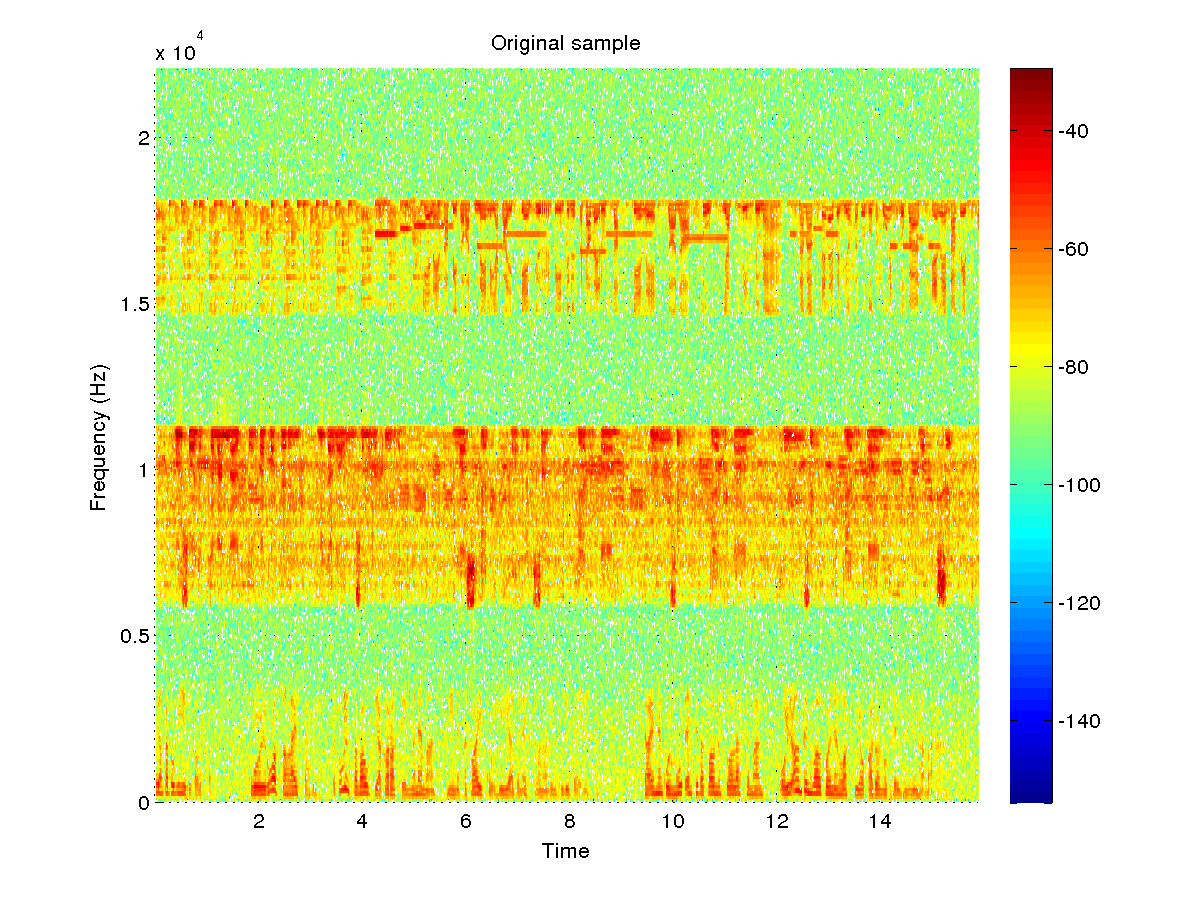
\includegraphics[width=180mm]{q1_spectrogram}
    \caption{Spectrogram of the signal. \label{fig:q1_spectrogram}}
  \end{center}  
\end{figure}

Assignment instructed the use of an IIR-filter with 500Hz transition
bands and maximum of 2 dB passband ripple.  The filter specification was
drawn with {\tt speksitIIR}, obtained from the course page.
